\documentclass[openany, parskip=full, 12pt, a4]{scrbook}

\usepackage[utf8]{inputenc}
\usepackage[T1]{fontenc}

%---------------------------------------------------------
% PACKAGES
%---------------------------------------------------------

% TYPOGRAPHY
\usepackage{xspace}
\usepackage{microtype}
\usepackage{cmbright} % different fonts

% VARIA
\usepackage{color}
\usepackage[table]{xcolor} % loads also »colortbl« %load before tikz if options
\usepackage{scrhack} % fix koma script warning about addtolist
\usepackage{blindtext}
\usepackage{pdfpages} % for cover 

\usepackage{ifthen} % to have online and printed versionw

% GRAPHICS & FIGURES & TABLES
\usepackage{graphicx}
\usepackage{float}
\usepackage{multicol} % for timetable
\usepackage{longtable} % for list of participants over more than 1 page
%\usepackage{wrapfig}
%\usepackage{tikz}
%\tikzset{ar/.style={>=latex, ->}}
%\renewcommand{\arraystretch}{1.2}
%\usepackage[multidot]{grffile}
% \usepackage{booktabs}

% WANTS TO BE LAST
\usepackage[english]{babel}

\usepackage[hidelinks]{hyperref}
\hypersetup{pdfpagelayout=TwoPageRight}
% \usepackage[ocgcolorlinks]{hyperref}
% \hypersetup{colorlinks, linkcolor={wolf}, linktocpage=true, citecolor ={tpred}, urlcolor={black}}


%-------------------------------------------------------------
% SETTINGS
%-------------------------------------------------------------
\pagestyle{plain}

\setcounter{secnumdepth}{-2} % remove numbering at any level both for the heading and the toc
%https://tex.stackexchange.com/questions/30122/generate-table-of-contents-when-section-sections-without-numbering-has-been




%-------------------------------------------------------------
% USEFUL DEFINTIONS
%-------------------------------------------------------------

% VARIA 
\newcommand\tab[1][1cm]{\hspace*{#1}}




% FOR THE TOC





%
% COLORS
%

\definecolor{myorange}{RGB}{255,117,40}
\definecolor{mygray}{RGB}{164, 168, 172}
\definecolor{mywhite}{RGB}{235, 238, 231}
\definecolor{myblue}{RGB}{52, 115, 116}

\newcommand{\primarycolor}{myblue}
\newcommand{\secondarycolor}{mywhite}
\newcommand{\ternarycolor}{mywhite}

%
% BOOKLET VERSIONS
%

% If compilation is done with 'compile.sh', both versions (online and printed) are automatically compiled
% If compilation is done from editor, choose which version to compile below
\makeatletter
\@ifundefined{ifOnline}{% % check if already defined from the command line, if not define \ifOnline
	\expandafter\newif\csname ifOnline\endcsname
	\Onlinefalse %set to \Onlinefalse/\Onlinetrue for printed/online version
}{}
\makeatother

% define \type to input the right version of the abstracts
\ifOnline
\newcommand{\type}{o}
\else
\newcommand{\type}{p}
\fi % end if

%
% ABSTRACT ENVIRONMENTS
%

%----------------------------------------
% online abstract environment
%----------------------------------------
\newenvironment{abstract_online}[4] %{title}{author}{affiliation}{type}
{\filbreak %avoid page break
	
	{\large \bfseries #1}
	
	{\bfseries \itshape #2} \hfill {#3}
	
	\textcolor{mygray}{#4}
	
}
{}

%----------------------------------------
% talk abstract environment (printed)
%----------------------------------------
\newenvironment{abstract}[4] %{title}{author}{affiliation}
{\filbreak %avoid page break
	
	{\large \bfseries #1}
	
	{\bfseries \itshape #2,} \textcolor{mygray}{#3} \hfill {#4}
	
	
}
{}

%----------------------------------------
% poster abstract environment (printed)
%----------------------------------------
\newcommand{\poster}[3] %{title}{author}{affiliation}
{\filbreak %avoid page break
	
	{\bfseries \large #1} \\	
	\tab #2, \textit{#3}
	
}
{}

%----------------------------------------
% tags for talk type (colored circle in abstracts)
%----------------------------------------

\newcommand{\KLtag}{\tikz[baseline={([yshift=-.8ex]current bounding box.center)}]  \node[circle, inner sep=2pt, minimum size=0.5em, color=black, fill=\KLcolor]{\small \bfseries KL};} %colored circle with tag

\newcommand{\IStag}{\tikz[baseline={([yshift=-.8ex]current bounding box.center)}]  \node[circle, inner sep=2pt, minimum size=0.5em, color=black, fill=\IScolor]{\small \bfseries IS};} %colored circle with tag

\newcommand{\CTtag}{\tikz[baseline={([yshift=-.8ex]current bounding box.center)}]  \node[circle, inner sep=2pt, minimum size=0.5em, color=black, fill=\CTcolor]{\small \bfseries CT};} %colored circle with tag

\newcommand{\ITtag}{\tikz[baseline={([yshift=-.8ex]current bounding box.center)}]  \node[circle, inner sep=2pt, minimum size=0.5em, color=black, fill=\ITcolor]{\small \bfseries IT};} %colored circle with tag


%
% PAGE LAYOUT DEFINITIONS
%
\usepackage{etoolbox}

%------------------------------------------------------
% page style: vertical line on the side of each page
%------------------------------------------------------
\usepackage[scale=1,angle=0,opacity=1]{background}
\backgroundsetup{contents={}}

\AddEverypageHook{%
\ifthenelse{%
	\isodd{\thepage} \AND  \thepage>1 % if odd page but not front page
	}{%
	\backgroundsetup{
		color=\secondarycolor,
		position=current page.south east,%
		nodeanchor=south east,
		contents={\rule{10pt}{0.66\paperheight}}
		}
	}{%
	% nothing
	}
%
\ifthenelse{% 
	\NOT \isodd{\thepage} \AND \NOT \thepage=44% if even page
	}{%
	\backgroundsetup{
		color=\secondarycolor,
		position=current page.south west,%
		nodeanchor=south west,
		contents={\rule{10pt}{0.66\paperheight}}
		}
	}{%
	% nothing
	}
\BgMaterial}


%---------------------------------------------------
% chapter heading style
%---------------------------------------------------

\newdimen\mybarpadding
\mybarpadding=1.5em\relax %padding between gcolored bar and chapter name

\RedeclareSectionCommand[%
    ,afterskip=4em plus 1pt minus 1pt%
    ,beforeskip=-1pt%1.2em plus 1pt minus 1pt%
    ,level=0%
    ,toclevel=0%
]{chapter}%

\setkomafont{chapter}{\normalfont\normalsize\bfseries\Huge} % koma-script-specific command

\newcommand*{\mynumberedtest}[1]{% to test whether there is a number
  \if\relax\detokenize{#1}\relax%
  \else%
    #1%
    
  \fi}

%-------------------------------------------------chapter style definition

\renewcommand{\chapterlinesformat}[3]{%
  \ifthispageodd{%
    \hfill%
    \raisebox{-0.2em}{%
      \makebox[0pt][r]{\textcolor{\primarycolor}{\rule{\paperwidth}{1em}}}%
    }%
    \hspace{\mybarpadding}%
% 	\mynumberedtest{#2}
	\mbox{#3}%
  }{%
%    \hbox{%
%       \mynumberedtest{#2}
      \mbox{#3}%
      \hspace{\mybarpadding}%
      \raisebox{-0.2em}{%
        \makebox[0pt][l]{\textcolor{\primarycolor}{\rule{\paperwidth}{1em}}}%
      }%
%    }%
  }%
}
\makeatother
%---------------------------------------------------------

% TIMETABLE COLORS AND STYLES

% text and backgroud colors
\newcommand{\tbg}{gray} % background
\newcommand{\tfg}{white}
\newcommand{\tbc}{gray!25}

% talk types colors
\newcommand{\IScolor}{myblue!65} % invited speaker
\newcommand{\CTcolor}{white} % contributed talk
\newcommand{\KLcolor}{myorange!45} % keynote lecture
\newcommand{\ITcolor}{yellow!25} %

% row types
\newcommand{\tablebreak}[2]{% {time span}{break name}
	\rowcolor{\tbc} #1 &  \multicolumn{4}{c|}{\bfseries #2} \\ \hline }
\newcommand{\eventtype}[2]{% {time span}{event name}
	#1& \multicolumn{4}{c|}{\cellcolor{\tbg}\color{\tfg}\bfseries #2} \\ \hline }

% column spacing and position
\newcolumntype{L}[1]{%
	>{\raggedright\let\newline\\\arraybackslash\hspace{0pt}}m{#1}}
\newcolumntype{C}[1]{%
	>{\centering\let\newline\\\arraybackslash\hspace{0pt}}m{#1}}
\newcolumntype{R}[1]{%
	>{\raggedleft\let\newline\\\arraybackslash\hspace{0pt}}m{#1}}

%\newcommand{\mytable}{|C{0.15\linewidth}| C{0.05\linewidth}|  C{0.25\linewidth} C{0.1\linewidth} C{0.5\linewidth}|}

\newcommand{\IS}[5]{% {time span}{name}{University}{City, Country}{title}
	#1 &\cellcolor{\IScolor}IS&{\bfseries#2}\newline #4&&#5 \\ \hline}
\newcommand{\CT}[5]{%
	#1 &\cellcolor{\CTcolor}CT&{\bfseries#2}\newline #4&&#5 \\ \hline}
\newcommand{\KL}[5]{%
	#1 &\cellcolor{\KLcolor}KL&{\bfseries#2}\newline #4&&#5 \\ \hline}
\newcommand{\IT}[5]{%
	#1 &\cellcolor{\ITcolor}IT&{\bfseries#2}\newline #4&&#5 \\ \hline}
\newcommand{\tutorial}[5]{%
	#1 && {\bfseries#2}\newline #4 &&#5 \\ \hline}
	
\begin{document}

\includepdf{cover}	
	
\mbox{}
\thispagestyle{empty}
\vfill
\begin{center}
	\ifOnline
	The electronic version of this booklet can be found at: \\
	https://amcosconference.com/
	\else
	This is the short version of the booklet for print use. Full abstracts with all authors, references, and figures can be found in the electronic version at \url{https://amcosconference.com/}
	\fi % end if
	\\[20pt]
	The codes used to generate this booklet, including the \LaTeX\space template, are available at \url{https://github.com/maximelucas/AMCOS\_booklet}
\end{center}

\newpage

\tableofcontents

\chapter{About}

{\small \textcolor{myblue}{This is a generic version of the real AMCOS conference booklet for which this \LaTeX{} template was generated. All information about the use and distribution of this template, and all related codes, can be found at \url{https://github.com/maximelucas/AMCOS\_booklet}.}}

\section{AMCOS}
The conference on Analysis and Modeling of Complex Oscillatory Systems (AMCOS) aims to bring together theoretical and experimental researchers working on the state of the art in the field of complex oscillatory systems.

The main topics of the conference comprise both (a) the modeling of complex systems and the emergence of collective behavior, as well as (b) the analysis of complex data sets in order to infer the underlying structure and functionality of networks. Particular focus will be put on oscillatory phenomena in neuroscience.

\section{COSMOS}

The AMCOS Conference is organized by the Early Stage Researchers (ESRs) of the Marie Curie Initial Training Network led by Arkady Pikovsky of Potsdam Univeristy. COSMOS trains 15 ESRs at the interface between Physics, Applied Mathematics, and Life Sciences, integrating theoretical and data-driven methods, in 7 universities across Europe.

\section{Organizing committee}
\begin{center}
\begin{tabular}{lll}
Gloria Cecchini & Marco Faggian &  Aleksandra Pidde \\
Rok Cestnik & R. Janis Goldschmidt &  Bastian Pietras\\
 Pau Clusella  & Marc Grau Leguia & Eero Satuvuori \\
 Nicolás Deschle & Maxime Lucas   &  Çağdaş Topçu \\
Federico Devalle  & Irene Malvestio  & Clément Zankoc 
\end{tabular}
\end{center}



% timetable ---------------------------------------------------------------------------
\chapter{Timetable}

CT: Contributed Talk, IS: Invited Speaker, KL: Keynote Lecture, IT: Invited Talk.

\section{Tuesday, 20 of March}
\begin{center}
	\filbreak
\begin{longtable}{|C{0.15\linewidth}| C{0.04\linewidth}|  C{0.3\linewidth} C{0.0\linewidth} C{0.4\linewidth}|}\hline	
	\tablebreak{8:30--9:00}{Registration}
	\tablebreak{9:00--9:10}{Welcome remarks}
	\KL{9:10--10:05}{Leon Tremblay}{}{Montreal, Canada}{Title of a keynote lecture}
	\CT{10:05--10:30}{Marc Fournier}{}{Brussels, Belgium}{Title of contributed talk}
	\tablebreak{10:30--11:00}{Coffee}
	\IS{11:00--11:40}{Hiroya Sato}{}{Tokyo, Japan}{Title of invited speaker}
	\CT{11:40--12:45}{Marc Smith}{}{Brussels, Belgium}{Title of contributed talk with math and paragraphs}
	\tablebreak{12:45--14:00}{Lunch}
	\CT{14:00--14:30}{Marc Rodriguez}{}{Barcelona, Spain}{Title of contributed talk with math and references}
	\IS{14:30--15:05}{Hiroya Sato}{}{Tokyo, Japan}{Title of invited speaker}
	\tablebreak{15:05--15:30}{Coffee}
	\CT{15:30-16:00}{Marc Jansen}{}{Amsterdam, The Netherlands}{Title of contributed talk and references and a figure}
	\IS{16:00-17:10}{Hiroya Sato}{}{Tokyo, Japan}{Title of invited speaker}
	\eventtype{17:10--19:30}{Poster session with Wine \& Cheese}
\end{longtable}
\end{center}

\newpage
\section{Wednesday, 21 of March}
\begin{center}
	\begin{longtable}{|C{0.15\linewidth}| C{0.04\linewidth}|  C{0.3\linewidth} C{0.0\linewidth} C{0.4\linewidth}|}\hline	
		\IS{9:00-9:40}{Hiroya Sato}{}{Tokyo, Japan}{Title of invited speaker}
		\CT{9:40-10:10}{Marc Fournier}{}{Brussels, Belgium}{Title of contributed talk}
		\IS{10:10--12:45}{Hiroya Sato}{}{Tokyo, Japan}{Title of invited speaker}
		\tablebreak{10:45--11:10}{Coffee}
		%odor
		\CT{11:10--11:40}{Marc Jansen}{}{Amsterdam, The Netherlands}{Title of contributed talk and references and a figure}
		\CT{11:40--12:10}{Marc Jansen}{}{Amsterdam, The Netherlands}{Title of contributed talk and references and a figure}
		\IS{12:10--12:45}{Hiroya Sato}{}{Tokyo, Japan}{Title of invited speaker}
		\tablebreak{12:45--14:00}{Lunch}
		\CT{14:00--14:30}{Marc Fournier}{}{Brussels, Belgium}{Title of contributed talk}
		\CT{14:30-15:00}{Marc Fournier}{}{Brussels, Belgium}{Title of contributed talk}
		\eventtype{16:30--18:00}{Excursion}
		\eventtype{20:00}{Conference Dinner}
	\end{longtable}
\end{center}

\newpage
\section{Thursday, 22 of March}
\begin{center}
	\begin{longtable}{|C{0.15\linewidth}| C{0.04\linewidth}|  C{0.3\linewidth} C{0.0\linewidth} C{0.4\linewidth}|}\hline	
		\IS{9:00 -- 9:40}{Hiroya Sato}{}{Tokyo, Japan}{Title of invited speaker}
		\IS{9:40--10:20}{Hiroya Sato}{}{Tokyo, Japan}{Title of invited speaker}
		\IT{10:20--10:45}{Franck Schmidt}{}{Munich, Germany}{A Special Talk about Diversity in Science}
		\tablebreak{10:45--11:10}{Coffee}
		\CT{11:10-11:40}{Marc Jansen}{}{Amsterdam, The Netherlands}{Title of contributed talk and references and a figure}
		\KL{11:40--12:35}{Leon Tremblay}{}{Montreal, Canada}{Title of a keynote lecture}
		\eventtype{12:35--12:45}{Poster Prize \& Conclusion}
		\tablebreak{12:45--14:00}{Lunch}
	\end{longtable}
\end{center}


% talks ---------------------------------------------------------------------------
\chapter{List of Abstracts -- Talks}

\section{Tuesday 20th}

\input{abstracts/tex/t\type_tremblay}
\input{abstracts/tex/t\type_fournier}
\input{abstracts/tex/t\type_sato}
\input{abstracts/tex/t\type_smith}
\input{abstracts/tex/t\type_rodriguez}
\input{abstracts/tex/t\type_jansen}

\section{Thursday 22nd}

\input{abstracts/tex/t\type_schmidt}
% posters ----------------------------------------------------------------------------------------------
\chapter{List of Posters} 

\vspace{-2.5em}

\section{Tuesday Session}


\input{abstracts/tex/p\type_doe}
\input{abstracts/tex/p\type_doe}
\input{abstracts/tex/p\type_doe}
\input{abstracts/tex/p\type_doe}
\input{abstracts/tex/p\type_doe}
\input{abstracts/tex/p\type_doe}
\input{abstracts/tex/p\type_doe}
\input{abstracts/tex/p\type_doe}


% list of participants
%----------------------------------------------------------------------------
\chapter{List of Participants}
 
\begin{center}
\rowcolors{1}{gray!25}{white}
\begin{longtable}{p{0.4\linewidth} p{0.4\linewidth} }
\hline
		John1 Doe1 & Barcelona, Spain \\ \hline
		John2 Doe2 & Barcelona, Spain \\ \hline
		John3 Doe3 & Barcelona, Spain \\ \hline
		John4 Doe4 & Barcelona, Spain \\ \hline
		John5 Doe5 & Barcelona, Spain \\ \hline
		John6 Doe6 & Barcelona, Spain \\ \hline
		John7 Doe7 & Barcelona, Spain \\ \hline
		John8 Doe8 & Barcelona, Spain \\ \hline
		John9 Doe9 & Barcelona, Spain \\ \hline
		John10 Doe10 & Barcelona, Spain \\ \hline
		John11 Doe11 & Barcelona, Spain \\ \hline
		John12 Doe12 & Barcelona, Spain \\ \hline
		John13 Doe13 & Barcelona, Spain \\ \hline
		John14 Doe14 & Barcelona, Spain \\ \hline
		John15 Doe15 & Barcelona, Spain \\ \hline
		John16 Doe16 & Barcelona, Spain \\ \hline
		John17 Doe17 & Barcelona, Spain \\ \hline
		John18 Doe18 & Barcelona, Spain \\ \hline
		John19 Doe19 & Barcelona, Spain \\ \hline
		John20 Doe20 & Barcelona, Spain \\ \hline
		John21 Doe21 & Barcelona, Spain \\ \hline
		John22 Doe22 & Barcelona, Spain \\ \hline
		John23 Doe23 & Barcelona, Spain \\ \hline
		John24 Doe24 & Barcelona, Spain \\ \hline
		John25 Doe25 & Barcelona, Spain \\ \hline
		John26 Doe26 & Barcelona, Spain \\ \hline
		John27 Doe27 & Barcelona, Spain \\ \hline
		John28 Doe28 & Barcelona, Spain \\ \hline
		John29 Doe29 & Barcelona, Spain \\ \hline
\end{longtable}
\end{center}
 

% venue + useful info ----------------------------------------------------------------------------
\chapter{Useful Information}

\textbf{Talks} will be held at the \textbf{Conference Hall-Auditorium} of PRBB. It is situated on the first floor of the central courtyard and
has independent access from the rest of the building (through stairs located at the ground floor, main entrance of PRBB). 

\textbf{Coffee breaks and lunches} will be offered in the half-covered terrace in front of the main entrance of the conference hall.

The \textbf{poster session} will be held on Tuesday and Wednesday night on the \textbf{ground floor} of the PRBB. 

Wi-Fi will be available during the conference. The PRBB also provides access to an eduroam network.

The \textbf{conference dinner} will be held at the "The best restaurant", at Some Street, 39, Barcelona.

\section{How to get to the PRBB?}

The PRBB building overlooks the Ronda del Litoral and is next to the twin towers of the Olympic Village: Torre Mapfre and Arts Hotel. The address is Carrer del Dr. Aiguader, 88, 08003 Barcelona, Spain. and and can be reached by:

\begin{itemize}

	\item \textbf{Subway:} yellow line, L4, station Ciutadella/Vila Ol\'{i}mpica,
	\item \textbf{Bus:} lines V21, 14, 36, 41, 45, 59, 71, 92, D20,
	\item \textbf{Tram:} line 4, stop Vila Ol\'{i}mpica.
	
\end{itemize}

\begin{center}
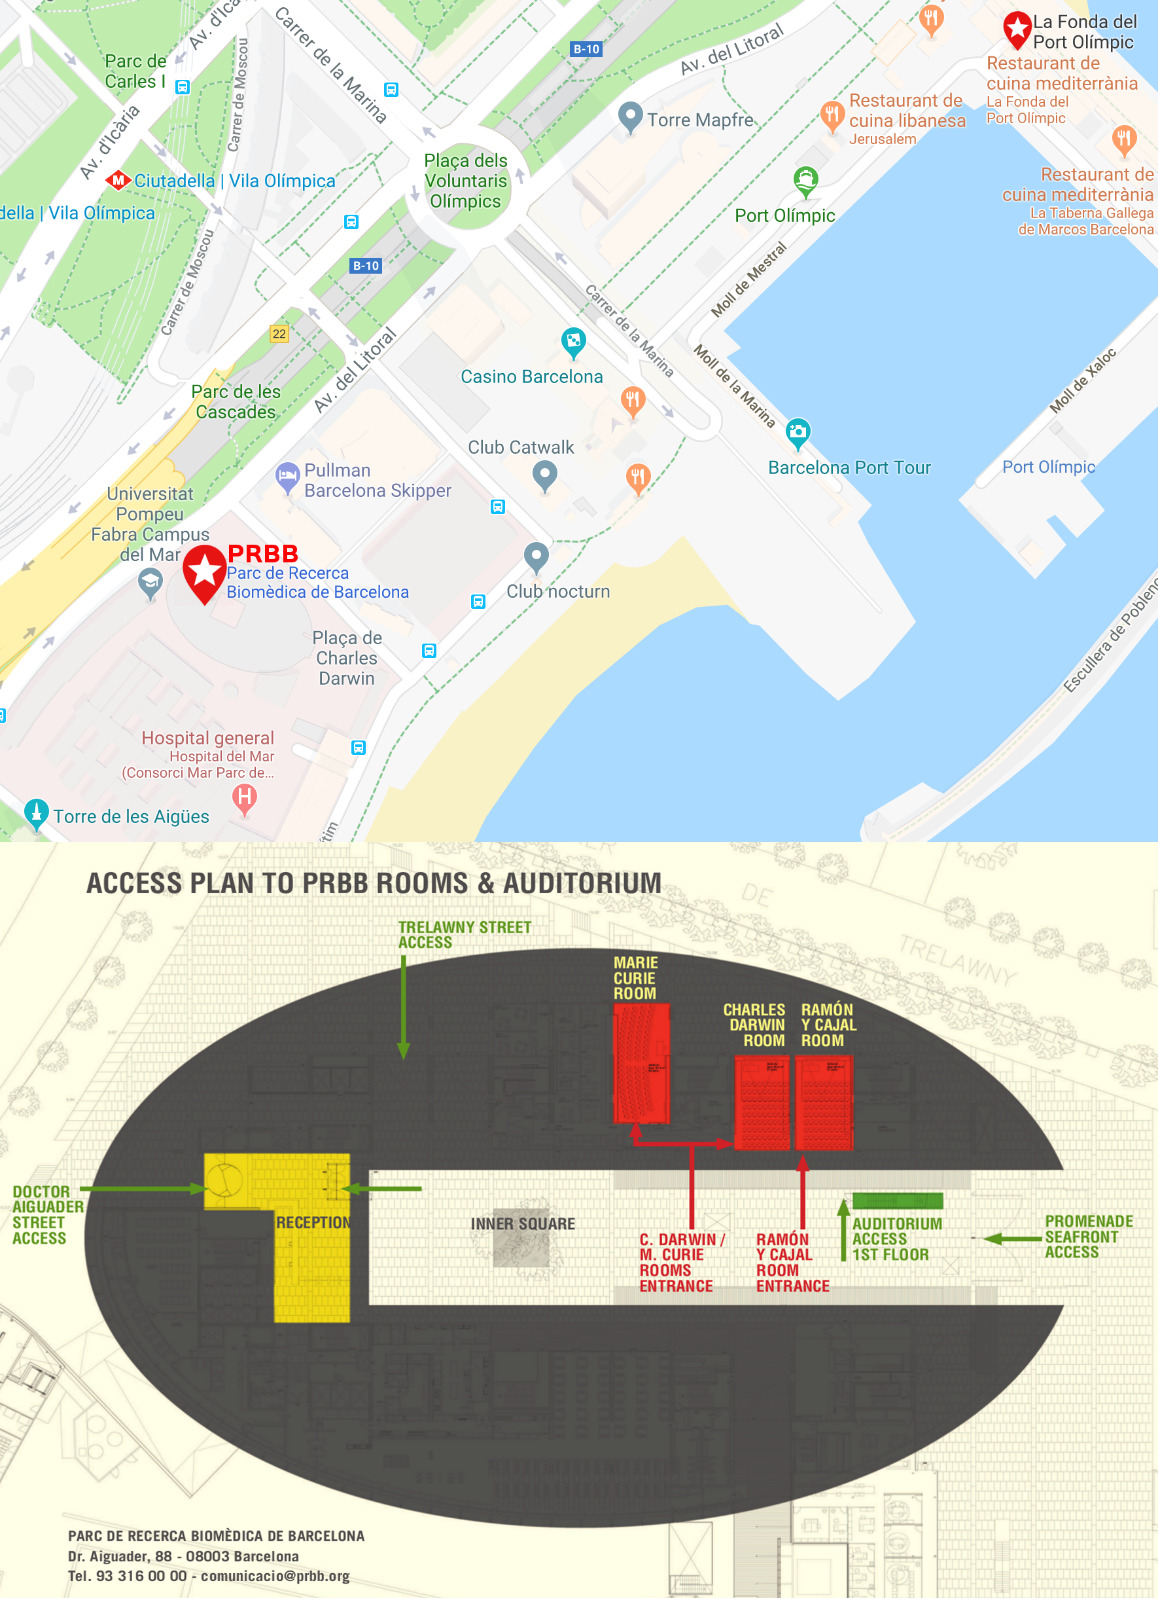
\includegraphics[width=\linewidth]{images/amcos_map}
\end{center}


\chapter{Partner Institutions and Sponsors}

\begin{center}
The AMCOS conference is part of the COSMOS project, funded by the European Union’s Horizon 2020 research and innovation programme under the Marie Sk\l{}odowska-Curie grant agreement No 642563.
\end{center}

\vfill

\section{Sponsors}

\begin{center}

\includegraphics[width=0.5\textwidth]{images/logos/Partnerlogos/LancasterHelium.jpg}
\includegraphics[width=0.5\textwidth]{images/logos/Partnerlogos/springer.pdf}
\end{center}

\vfill


\newpage

\pagecolor{myblue}
\thispagestyle{empty}
\mbox{}

\end{document}
